
\begin{frame}{Decay Channels}
  \begin{minipage}[c][\textheight]{0.45\textwidth}
    \begin{itemize}
        %TODO: Check the limits on non-bW decays
      \item<1-> All* tops will immediately decay to a b-quark and a W-boson
      \item<2-> The W-boson will immediately decay either
        \begin{itemize}
          \item<2,4-> \textbf{Leptonically}
          \item<3-> \textbf{Hadronically}
        \end{itemize}
      \item<4-> The b-quark will form some b hadron, travel some macroscopic distance, and then hadronize into a jet.
    \end{itemize}
  \end{minipage}
  \begin{minipage}[c][\textheight]{0.54\textwidth}
    \centering
    \only<1>{%
      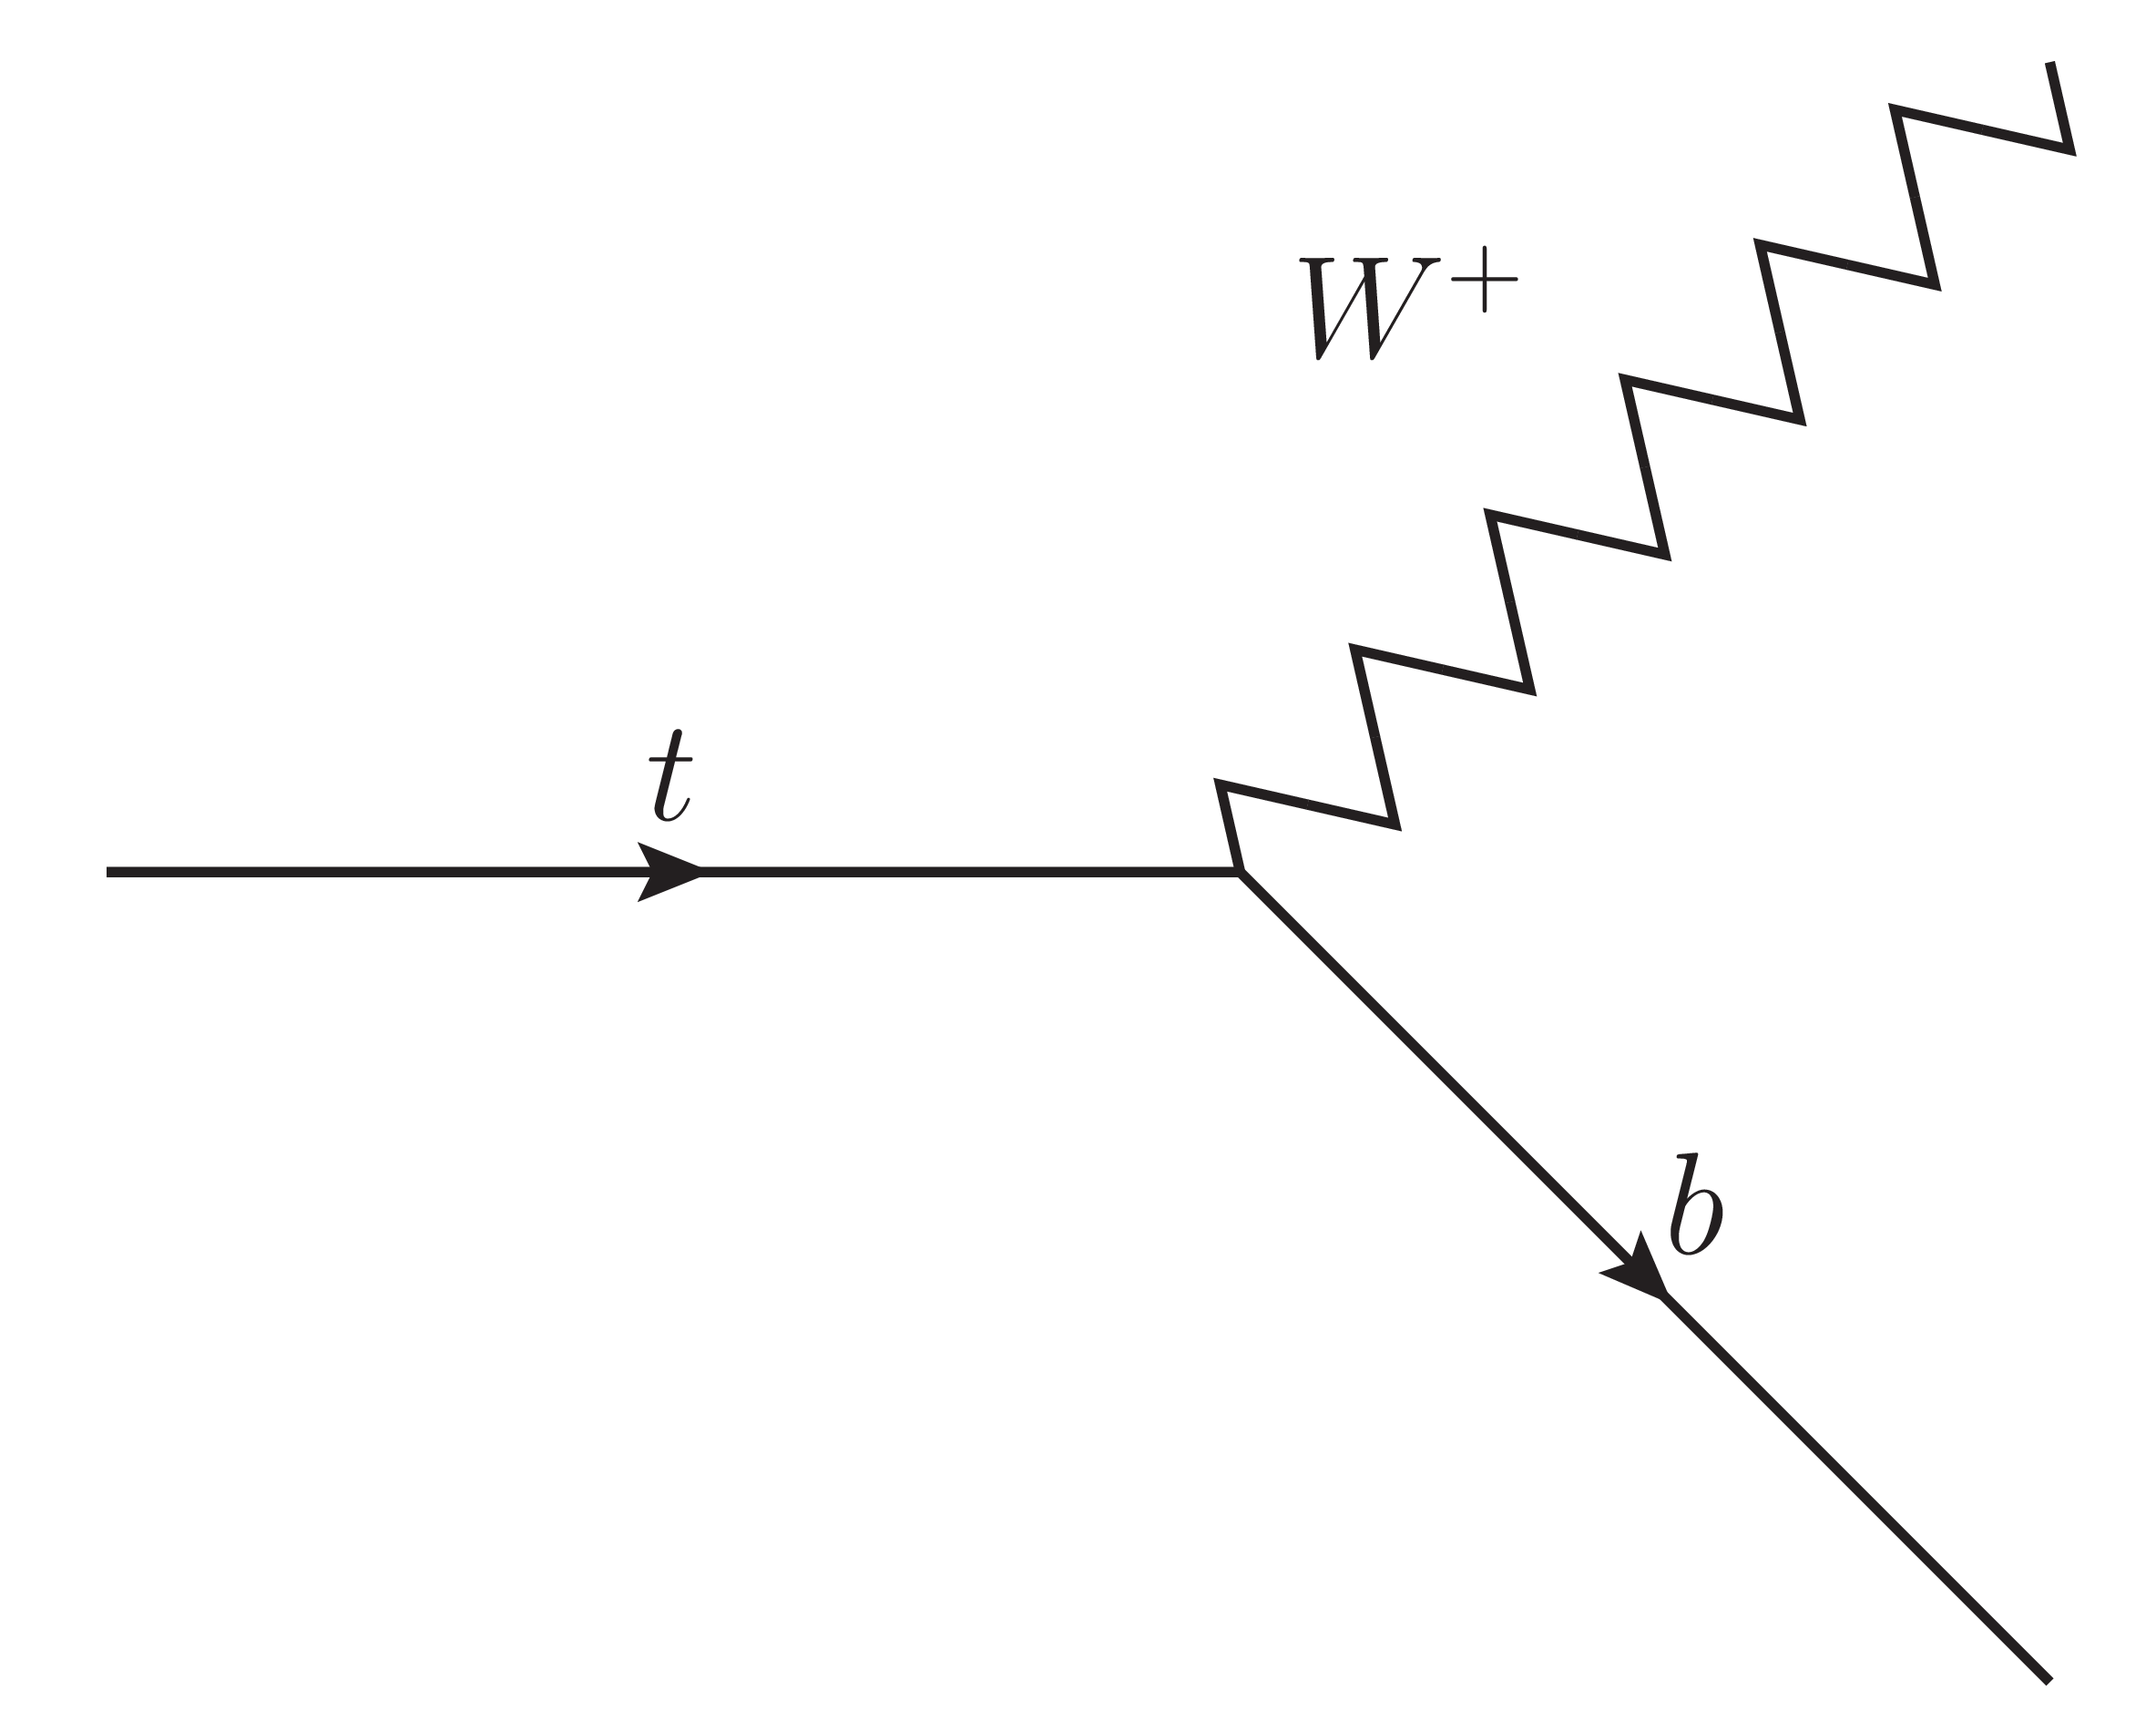
\includegraphics[width=\textwidth]{figures/feynman-diagrams/T-b_W.png}
    }
    \only<2>{%
      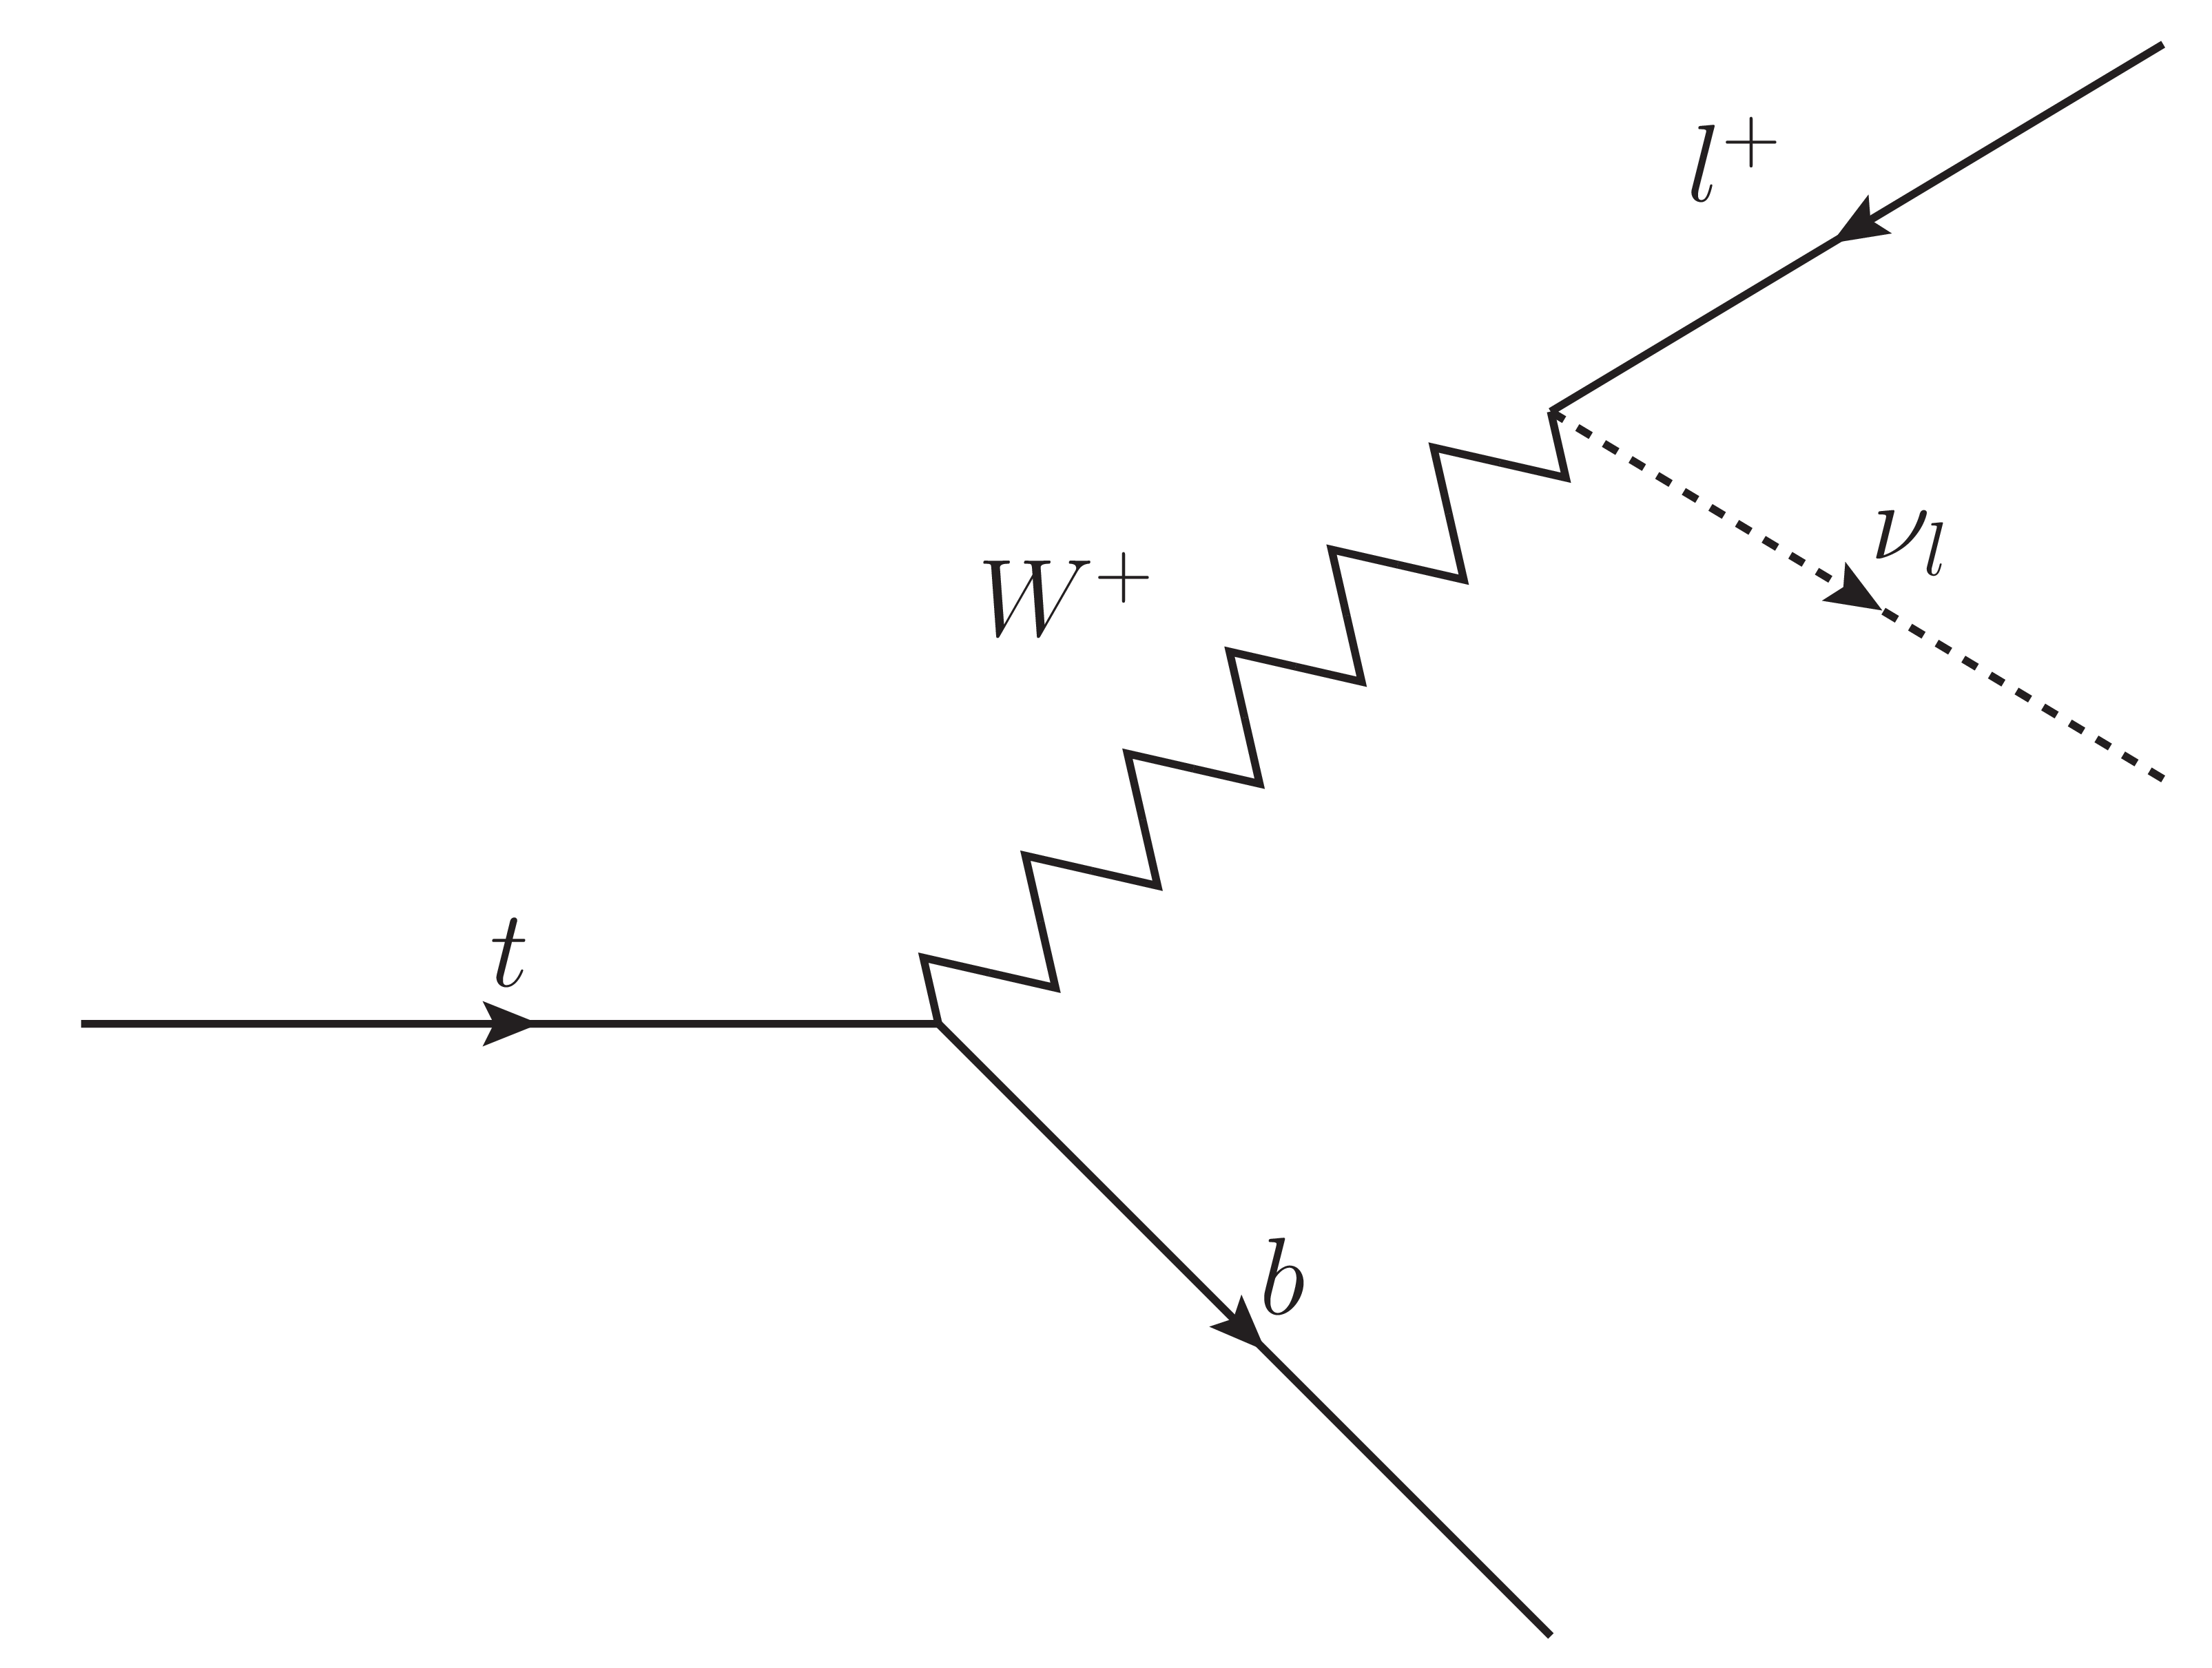
\includegraphics[width=\textwidth]{figures/feynman-diagrams/T-b_W-ln.png}
    }
    \only<3>{%
      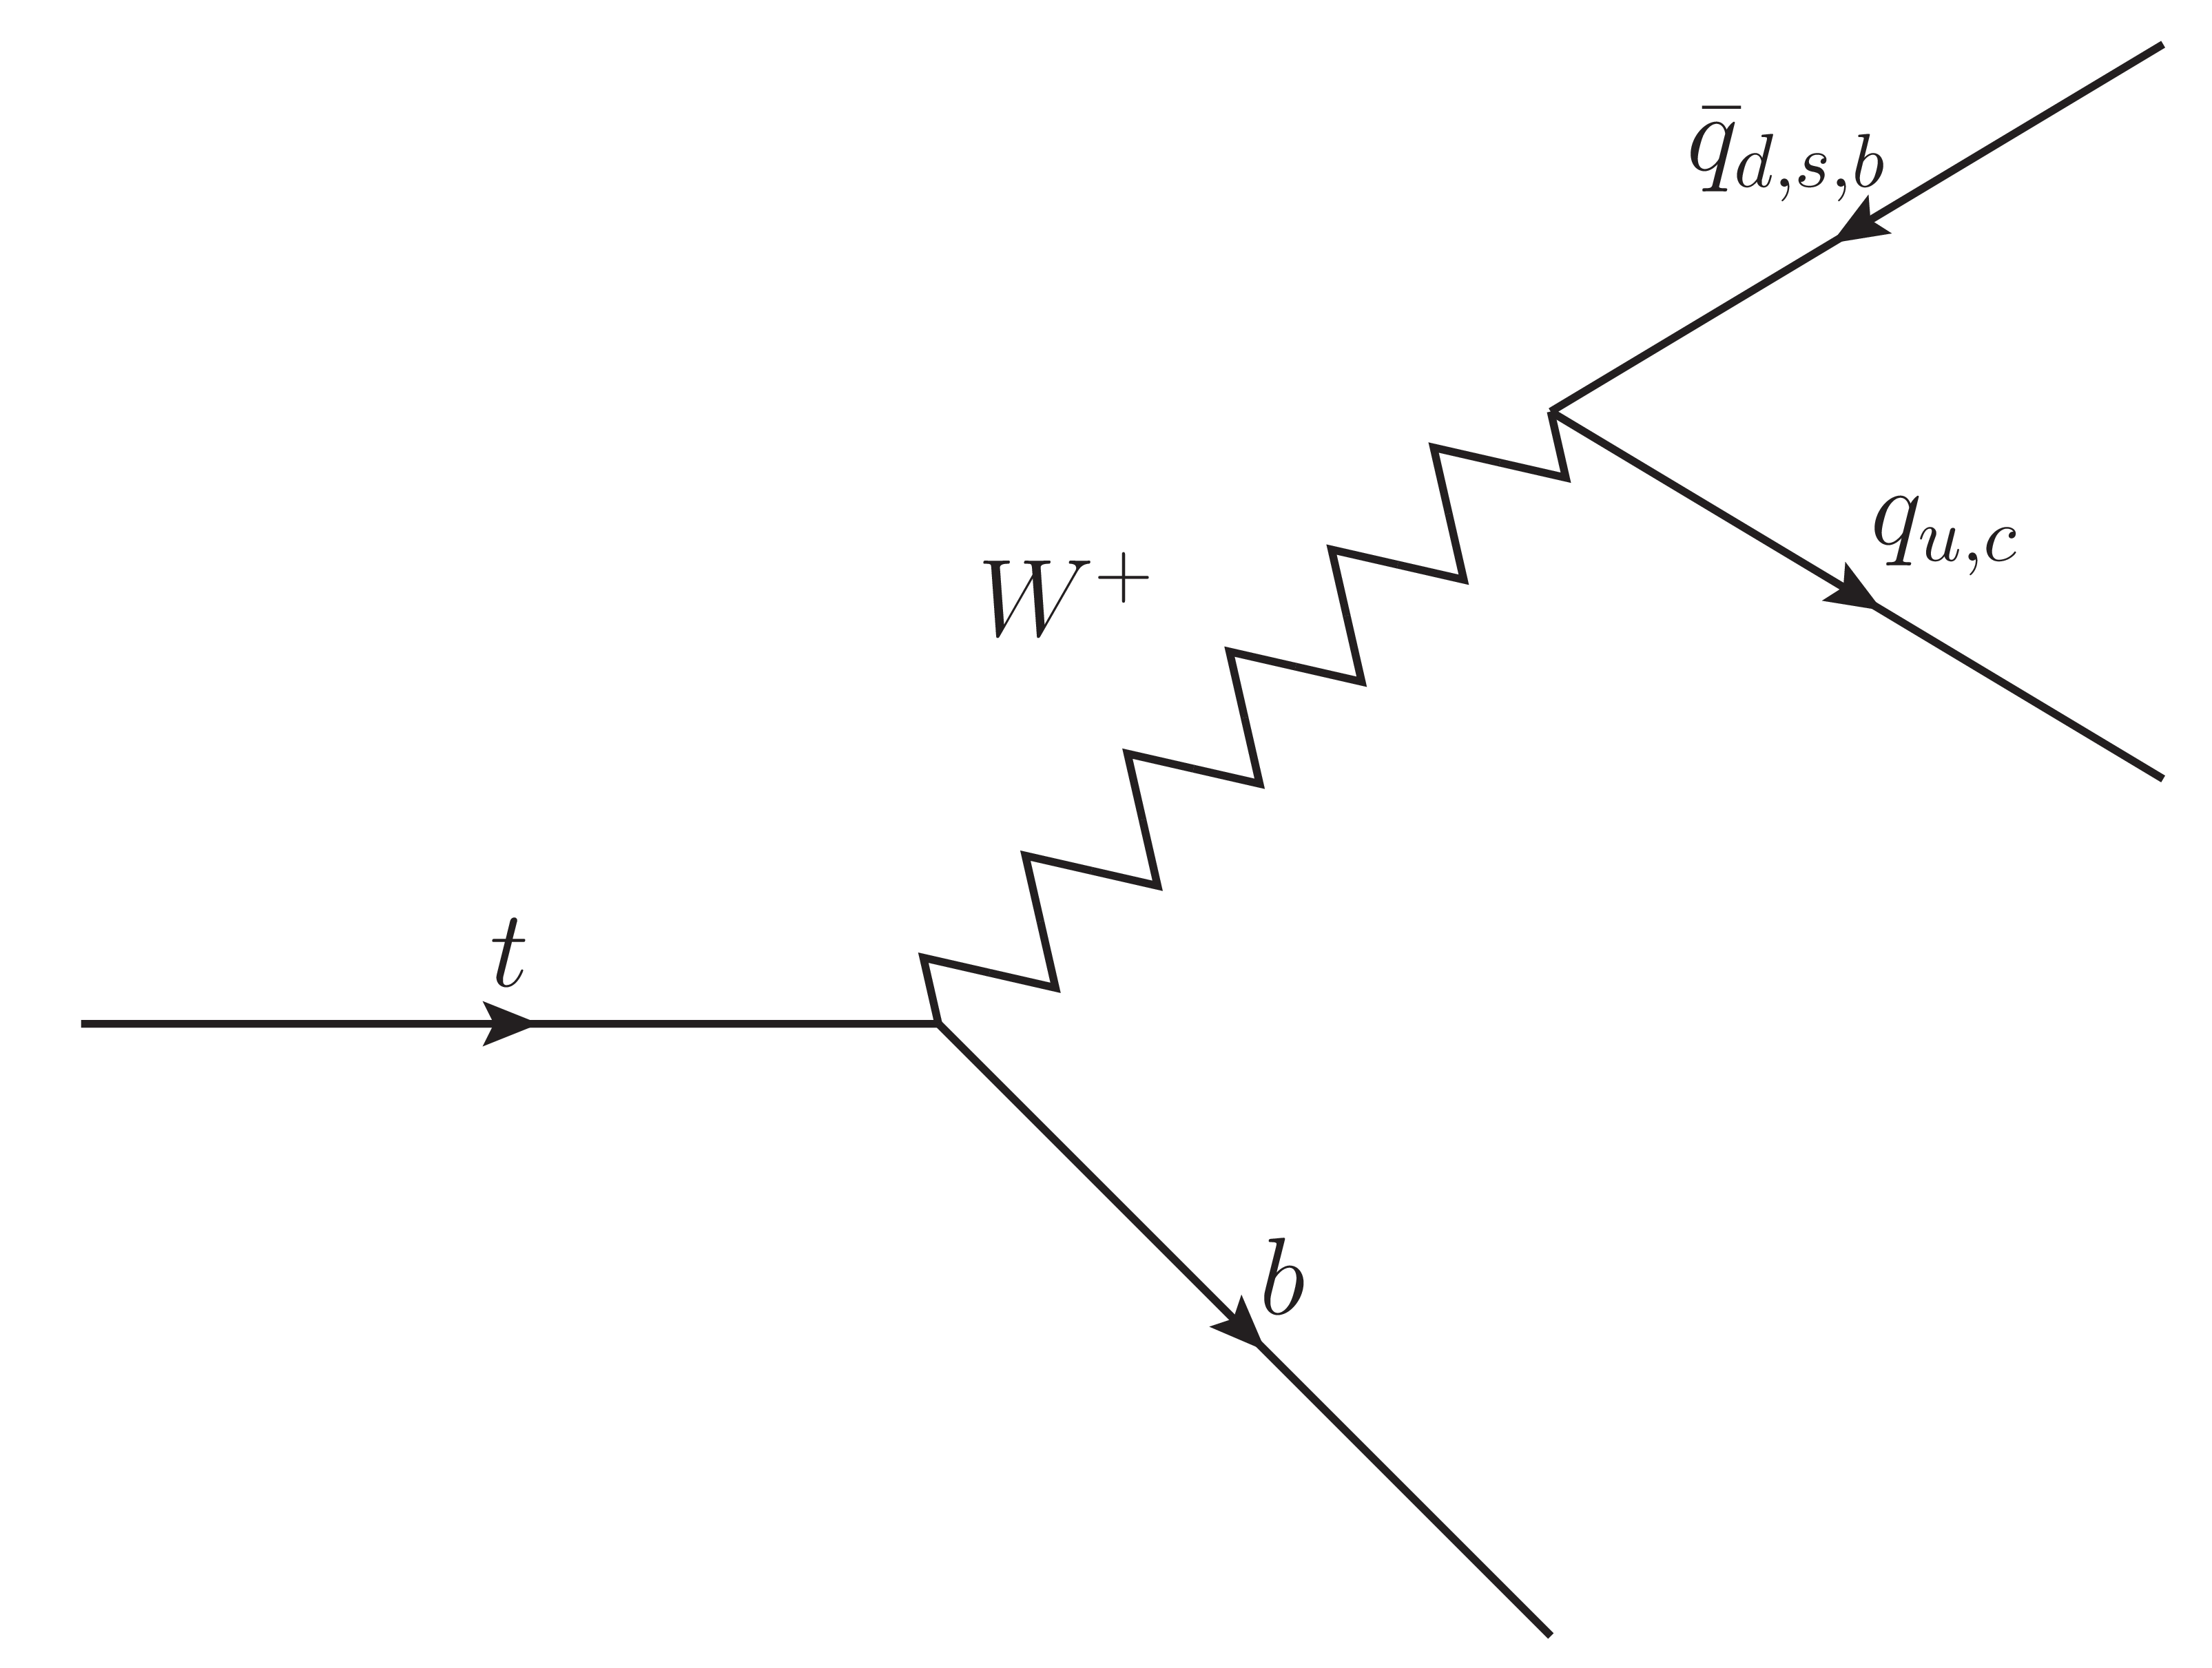
\includegraphics[width=\textwidth]{figures/feynman-diagrams/T-b_W-qq.png}
    }
    \only<4>{%
      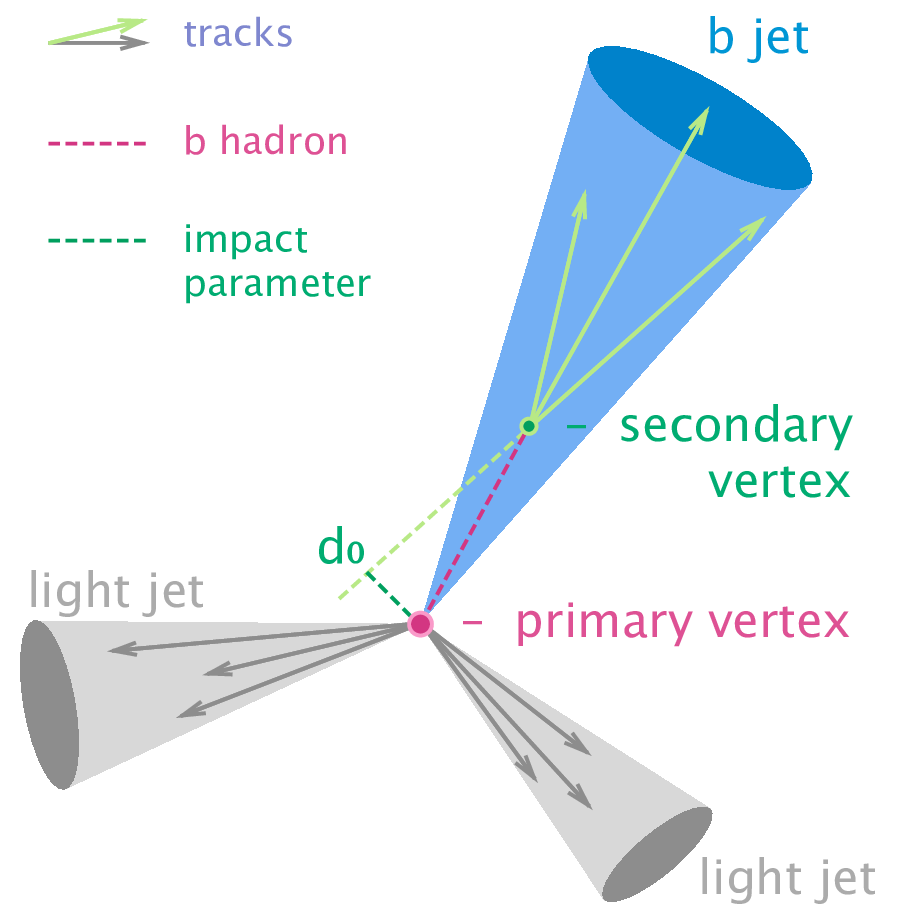
\includegraphics[width=0.90\textwidth]{figures/b-tagging}
    }
  \end{minipage}
\end{frame}
